\documentclass[14pt,a4paper]{scrartcl}
\usepackage{cmap}
\usepackage[utf8]{inputenc}
\usepackage[T1,T2A]{fontenc}
\usepackage[english,russian]{babel}
\usepackage{relsize}
\usepackage{graphicx}
\usepackage{subfigure}
\usepackage{mathtools}
\usepackage{amssymb}
\usepackage{float}
\usepackage{sidecap}
\usepackage{wrapfig}
\usepackage{caption}
\usepackage[table,xcdraw]{xcolor}
\usepackage{minted}
\usepackage{tcolorbox}
\usepackage{enumitem}
\makeatletter

\renewcommand{\thesubsection}{\arabic{subsection}}

\newenvironment{sqcases}{%
	\matrix@check\sqcases\env@sqcases
}{%
	\endarray\right.%
}
\def\env@sqcases{%
	\let\@ifnextchar\new@ifnextchar
	\left\lbrack
	\def\arraystretch{1.2}%
	\array{@{}l@{\quad}l@{}}%
}
\makeatother

\begin{document}
	\begin{titlepage}
	\begin{center}
		\large
		МИНИСТЕРСТВО ОБРАЗОВАНИЯ И НАУКИ\\ РОССИЙСКОЙ ФЕДЕРАЦИИ
		
		\vspace{0.5cm}
		
		МГТУ им Н.Э.Баумана
		\vspace{0.25cm}
		
		Факультет ФН
		
		Кафедра вычислительной математики и математической физики
		\vfill
		
		
		Соколов Арсений Андреевич\\
		\vfill
		
		
		{\LARGE Семинар от 25.04.20\\ по основам сеточных методов \\[2mm]
		}
		\bigskip
		
		3 курс, группа ФН11-63Б\\
		Вариант 3
	\end{center}
	\vfill
	
	\newlength{\ML}
	\settowidth{\ML}{«\underline{\hspace{0.7cm}}» \underline{\hspace{2cm}}}
	\hfill\begin{minipage}{0.4\textwidth}
		Преподаватель\\
		\underline{\hspace{3cm}} В.\,А.~Кутыркин\\
		«\underline{\hspace{0.7cm}}» \underline{\hspace{1.71cm}} 2020 г.
	\end{minipage}%
	\bigskip
	
	
	\vfill
	
	\begin{center}
		Москва, 2020 г.
	\end{center}
\end{titlepage}
Семинар от 25.04.2020, Основы сеточных методов , ФН11-63Б, вариант 3,
Соколов Арсений Андреевич, Кутыркин Владимир Андреевич

\section*{Задачи для решения на семинаре}

\textbf{Задача1.} На рисунке $1$ показан шаблон внутреннего узла трёхслойной неявной конечно разностной схемы для уравнения колебания струны (\ref{1}). Исследовать спектральную устойчивость этой неявной схемы.
 
\begin{figure}[H]
	\begin{minipage}[h]{1\linewidth}
		\center{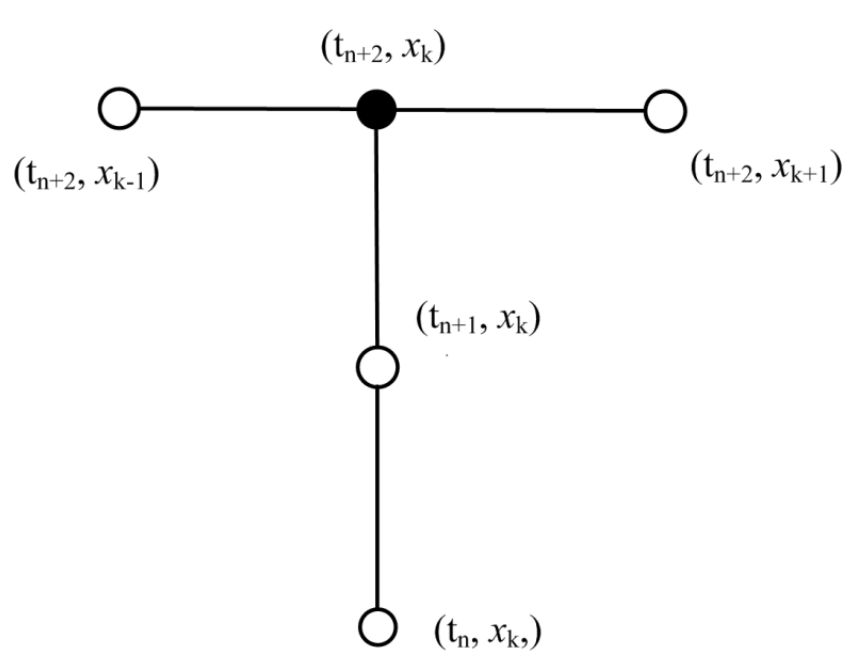
\includegraphics[width=.7\linewidth]{../img/ris_1.png}}
	\end{minipage}
\end{figure}


\begin{equation}\label{1}
	\left\{\begin{array}{l}
	\frac{\partial^{2} u(t, x)}{\partial t^{2}}-\frac{\partial^{2} u(t, x)}{\partial x^{2}}=f(t, x),(t, x) \in(0, T) \times \mathbb{R} \\
	u(0, x)=\mu(x), \quad x \in \mathbb{R}, \frac{\partial u}{\partial t}(0, x)=\eta(x) \quad (\textup{начальные условия}),
	\end{array}\right.
\end{equation}

где $u \in C([0 ; T], \mathbb{R})$ -- неизвестная гладкая функция, $\mu \in C(\mathbb{R}, \mathbb{R})$, и \\$f \in C([0 ; T] \times \mathbb{R}, \mathbb{R})$ -- заданные гладкие функции.


\textbf{Решение.}

Неявная разностная схема для задачи (\ref{1}), индуцированная для внутреннего узла сетки $C$ с шаблоном, показанным на рисунке $1$, определяет аппроксимирующую задачу (\ref{1}) (тип аппроксимирования $(\tau^2, h^2)$) конечно разностную схему:

\begin{equation*}
	\left\{\begin{array}{l}
	\frac{u_{k}^{n}-2 u_{k}^{n+1}+u_{k}^{n+2}}{\tau^{2}}-\frac{u_{k+1}^{n+2}-2 u_{k}^{n+2}+u_{k-1}^{n+2}}{h^{2}}=f_{k}^{n+2}, N=\overline{1, n-1}, k \in Z \\
	u_{k}^{0}=\mu_{k}, \frac{u_{k}^{1}-u_{k}^{0}}{\tau}=\eta_{k}, k \in Z
	\end{array}\right.
\end{equation*}


Для исследования спектральной устойчивости трёхслойной схемы также можно использовать спектральный признак устойчивости, анализируя конечно разностную схему вида:

\begin{equation*}
	\frac{u_{k}^{n}-2 u_{k}^{n+1}+u_{k}^{n+2}}{\tau^{2}}-\frac{u_{k+1}^{n+2}-2 u_{k}^{n+2}+u_{k-1}^{n+2}}{h^{2}}=f_{k}^{n+2}, N=\overline{1, n-1}, k \in Z,
\end{equation*}

где, согласно спектральному признаку, используются соотношения:

\begin{align*}
	&u_{k}^{n}=e^{i \varphi k}, \varphi \in[0 ; 2 \pi) ; \quad u_{k}^{n}=\lambda u_{k}^{n-1}, u_{k}^{n+1}=\lambda u_{k}^{n}=\lambda^{2} u_{k}^{n-1}, k \in Z, \\
	&r=\frac{\tau^{2}}{h^{2}}, e^{i \varphi}-2+e^{-i \varphi}=-4 \sin ^{2}\left(\frac{\varphi}{2}\right)
\end{align*}


Получаем:
\begin{equation*}
	\lambda^{2}\left(1+4 r \sin ^{2}\left(\frac{\varphi}{2}\right)\right)-2 \lambda+1=0
\end{equation*}


Из теоремы Виета, получаем:

\begin{equation*}
	\left\{\begin{array}{l}
	\lambda_{1}+\lambda_{2}=-\frac{b}{a}; \\
	\lambda_{1} \cdot \lambda_{2}=\frac{c}{a}.
	\end{array}\right.
\end{equation*}

\begin{equation*}
	\Downarrow
\end{equation*}


\begin{equation*}
	\left\{\begin{array}{l}
	\lambda_{1}+\lambda_{2}=\frac{2}{1+4 r \sin ^{2}\left(\frac{\varphi}{2}\right)}; \\
	\lambda_{1} \cdot \lambda_{2}=\frac{1}{1+4 r \sin ^{2}\left(\frac{\varphi}{2}\right)}.
	\end{array}\right.
\end{equation*}

Откуда, решая полученную систему относительно $\lambda_{1}, \lambda_{2}$, имеем:

\begin{equation*}
	\left\{\begin{array}{l}
	\lambda_{1}=\frac{1+2 i \sqrt{r} \sin \left(\frac{\varphi}{2}\right)}{1+4 r \sin ^{2}\left(\frac{\varphi}{2}\right)}; \\
	\lambda_{2}=-\frac{1-2 i \sqrt{r} \sin \left(\frac{\varphi}{2}\right)}{1+4 r \sin ^{2}\left(\frac{\varphi}{2}\right)}.
	\end{array}\right.
\end{equation*}


Условие спектральной устойчивости неявной конечноразностной схемы для гиперболического уравнения колебания струны:

\begin{equation*}
	|\lambda|=\frac{1}{\sqrt{1+4 r \sin ^{2}\left(\frac{\varphi}{2}\right)}} \leq 1
\end{equation*}


То есть, неявная конечноразностная схема спектральной устойчива $\Rightarrow$ не накладывай ограничений на уменьшающиеся шаги сетки.


\pagebreak

\textbf{Задача 2.} Исследовать на спектральную устойчивость явную конечноразностную схему для матричной задачи (\ref{2})

\begin{equation}\label{2}
	\left\{\begin{array}{l}
	\frac{\partial^{>} \boldsymbol{w}}{\partial t}-\boldsymbol{A} \frac{\partial^{>} \boldsymbol{w}}{\partial x}=^{>} \mathbf{0}, \quad(t, x) \in(0 ; T] \times \mathbb{R} ; \\
	^>\boldsymbol{w}(0, x)=\mathbf{\Phi}(x), \quad x \in \mathbb{R}
	\end{array}\right.
\end{equation}
где 

\begin{equation*}
	A=\left(\begin{array}{ll}
	0 & 1 \\
	1 & 0
	\end{array}\right),
\end{equation*}

если на сетке $C$ эта схема имеет вид:

\begin{equation*}
	\left\{\begin{array}{l}
	\frac{^{>} w_{k}^{n+1}-^{>} w_{k}^{n}}{\tau}-A \frac{^{>} w_{k+1}^{n}-^{>} w_{k}^{n}}{2 h}=^{>} \mathbf{0}, N=\overline{1, n-1}, k \in \mathbb{Z} \\
	^{>} w_{k}^{0}=^{>} \Phi_{k}, \quad k \in \mathbb{Z}
	\end{array}\right.
\end{equation*}


\textbf{Решение.}

Согласно признаку спектральной устойчивости, для данной схемы рассматривается схема:

\begin{equation*}
	\frac{\lambda-1}{\tau}-A \frac{e^{i \varphi}-1}{2 h}=0,
\end{equation*}

где $^>w_k^n=^>de^{i\varphi k} \quad (^>g \in ^>\mathbb{R}^2, \quad ^>g\neq^>0), \varphi \in \left[0;2\pi\right)$

Подставляя $\forall \varphi \in \left[0;2\pi\right)$, получим:

\begin{equation*}
	\frac{\lambda-1}{\tau} {^>g} -A \frac{e^{i \varphi}-1}{2 h}{^>g}=^>0
\end{equation*}


Используя для числа Куранта обозначение: $r = \frac{\tau}{h}$:

\begin{equation*}
	\left[(\lambda-1) E-r A \frac{e^{i \varphi}-1}{2}\right] {^{>}} g={^{>}} 0
\end{equation*}

Если при умножении матрицы на ненулевой вектор в результате получен нулевой вектор, то это означает, что определитель матрицы равен нулю.

\begin{equation*}
	\left|\begin{array}{cc}
	\lambda-1 & -r \frac{e^{i \varphi}-1}{2} \\
	-r \frac{e^{i \varphi}-1}{2} & \lambda-1
	\end{array}\right|=(\lambda-1)^{2}-r^{2} \frac{\left(e^{i \varphi}-1\right)^{2}}{4}=0
\end{equation*}

\begin{equation*}
	\Downarrow
\end{equation*}

\begin{align*}
	\lambda_{1}(\varphi)=1+r \frac{e^{i \varphi}-1}{2},\\
	\lambda_{2}(\varphi)=1-r \frac{e^{i \varphi}-1}{2}
\end{align*}


Корни $\lambda_{1}(\varphi), \quad \lambda_{2}(\varphi)$ при изменении вещественного параметра $\varphi$ пробегают окружности радиуса $\frac{r}{2}$ с центрами в точках $1 - \frac{r}{2}$ и $1 + \frac{r}{2}$. Таким образом, условие устойчивости не выполнено ни при каких $r$

\begin{figure}[H]
	\begin{minipage}[h]{1\linewidth}
		\center{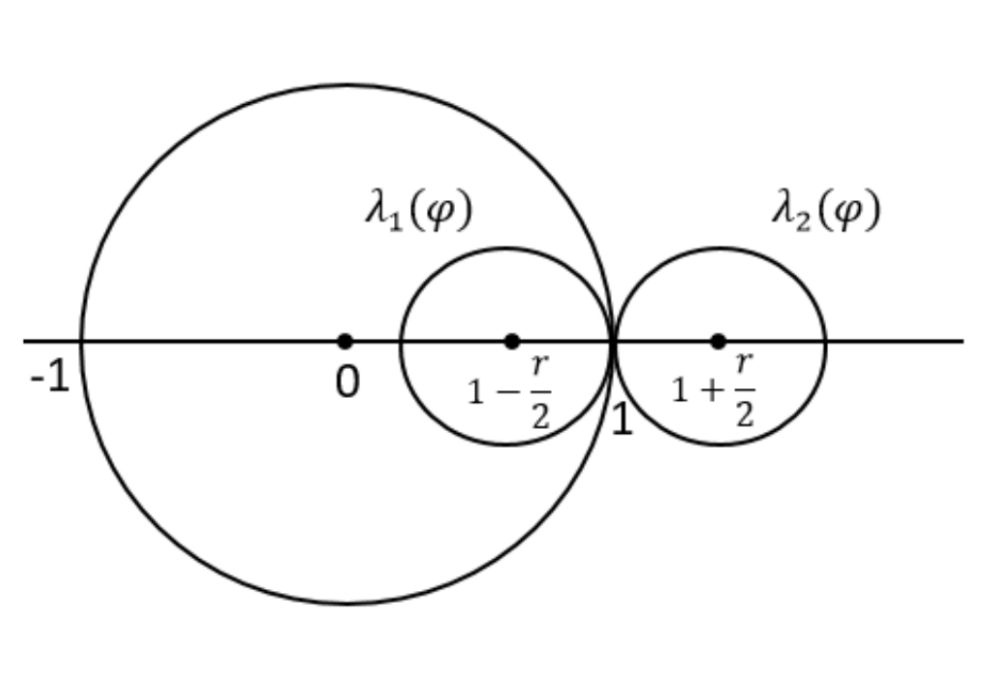
\includegraphics[width=.7\linewidth]{../img/ris_2.png}}
	\end{minipage}
\end{figure}







































\end{document}